%% ----------------------------------------------------------------
%% Thesis.tex -- MAIN FILE (the one that you compile with LaTeX)
%% ---------------------------------------------------------------- 

% Set up the document
\documentclass[a4paper, 11pt, oneside]{Thesis}  % Use the "Thesis" style, based on the ECS Thesis style by Steve Gunn
\usepackage[utf8]{inputenc}
\usepackage{verbatim}

\graphicspath{Figures/}  % Location of the graphics files (set up for graphics to be in PDF format)

% Include any extra LaTeX packages required
\usepackage{natbib}
\bibliographystyle{chicago}
\setcitestyle{authoryear,open={(},close={)}}
\usepackage{verbatim}  % Needed for the "comment" environment to make LaTeX comments
\usepackage{vector}  % Allows "\bvec{}" and "\buvec{}" for "blackboard" style bold vectors in maths
\hypersetup{urlcolor=blue, colorlinks=true}  % Colours hyperlinks in blue, but this can be distracting if there are many links.

% packages included by the author
\usepackage[portuguese]{babel}
\usepackage[inline]{enumitem}
\usepackage{pslatex}
\usepackage{tabularx}
% \usepackage{achicago}

\makeatletter
\newenvironment{tablehere}
  {\def\@captype{table}} {}
 
\newenvironment{figurehere}
  {\def\@captype{figure}}
  {}
\makeatother 

\begin{document}

\begin{center}
 \pagenumbering{roman}
\thispagestyle{empty}
\Large Danilo Augusto Silva \\[3.5cm] 
\textbf{\huge Circulação Gerada por Ventos Anômalos na Plataforma Continental Sudeste Durante o Verão de 2014. } 
\ \\ \ 

\bigskip\bigskip\bigskip\bigskip\bigskip\bigskip\bigskip\bigskip

\begin{flushright}
  \begin{minipage}{8cm}
  \small Primeiro relatório anual apresentado ao Instituto Oceanográfico da Universidade de São Paulo, como parte dos requisitos
  para o curso de Mestrado, no programa de Oceanografia, área de concentração Oceanografia Física. Período 2017/2019. \\ \ \\
  Orientador: Prof. Paulo Simionatto Polito\\ \ \\ \ \\ \ \\
  \end{minipage}
\end{flushright}

\ \\[3cm] São Paulo \\ Janeiro/2018
\end{center} 
 
\selectlanguage{brazil}

%% ----------------------------------------------------------------
%\lhead{\emph{Contents}}  % Set the left side page header to "Contents"
\tableofcontents  % Write out the Table of Contents

%% ----------------------------------------------------------------
\lhead{\emph{Lista de Figuras}}  % Set the left side page header to "List if Figures"
\listoffigures  % Write out the List of Figures

%% ----------------------------------------------------------------
\lhead{\emph{Lista de Tabelas}}  % Set the left side page header to "List of Tables"
\listoftables  % Write out the List of Tables

%% ----------------------------------------------------------------
% End of the pre-able, contents and lists of things
% Begin the Dedication page

%% ----------------------------------------------------------------
\mainmatter	  % Begin normal, numeric (1,2,3...) page numbering
\pagestyle{fancy}  % Return the page headers back to the "fancy" style

% Include the chapters of the thesis, as separate files
% Just uncomment the lines as you write the chapters

\lhead{\emph{Capítulo 1 - Atividades Realizadas}} 
\chapter{Atividades Realizadas}

\section{Disciplinas Cursadas}

\hspace{5mm} 

\begin{enumerate}
    \item Disciplina obrigatória - IOC5815 Dinâmica de Fluidos Geofísicos I;
    \item Disciplina obrigatória - IOC5811 Dinâmica de Fluidos Geofísicos II;
    \item Disciplina - IOC5817 Métodos de Análise de Dados Quase-Sinóticos em Oceanografia Física;
    \item Disciplina - Preparação Pedagógica em Oceanografia (FEA USP);
    \item Disciplina - IOC 5808 Cinemática e Dinâmica de Estuários
    \item Disciplina - IOC 5809 Hidrodinâmica da Plataforma Continental;
    \item Disciplina - IOC 5807 Modelos Numéricos Aplicados a Processos Costeiros e Oceânicos;
    \item Revisão Bibliográfica;
\end{enumerate}

\hspace{5mm} Além das disciplinas o que mais foi feito ??


\lhead{\emph{Capítulo 2 - Cronograma}} 
\chapter{Cronograma}
\label{cha:schedule}

\begin{enumerate}
    \item Revisão Bibliográfica;
    \item Obtenção, tratamento e análise de dados de vento;
    \item Elaboração de climatologia de vento;
    \item Implementação do modelo na PCSE;
    \item Simulações numéricas;
    \item Validação, comparação e análise dos resultados;
    \item Confecção da dissertação e de artigo científico referente aos resultados
    de modelagem numérica;
\end{enumerate}

\begin{tablehere}
\centering
\caption{Cronograma de atividades.}
\label{my-label}
\begin{tabular}{|c|c|c|c|c|c|c|c|c|c|c|c|c|}
\hline
\textbf{}     & Jan & Fev & Mar & Abr & Mai    & Jun & Jul    & Ago   & Set & Out & Nov & Dez   \\ \hline
2$^o$ ano (2018) & 1,2 & 1,3 & 4  & 4  & 4, 5 & 5  & 5, 6 & 6    & 7  & 7  & 7  & 7    \\ \hline
\end{tabular}
\end{tablehere}
\bigskip

Além das atividades citadas, relacionadas ao projeto de dissertação de mestrado, ainda serão executadas as seguintes atividades:

\begin{enumerate}
    \item Monitoria - Disciplina: IOF0201 - Fundamentos de Oceanografia Fisica (graduação, optativa), durante o primeiro semestre de 2018 e
    \item Monitoria - Disciplina: IOF0114 - Oceanografia Física Costeira e Estuarina (graduação, obrigatória), durante o segundo semestre de 2018.
\end{enumerate}

% \lhead{\emph{Anexo A - Introdução}} 
% \chapter{Introdução}

\section{Área de Estudo}
\label{sec:studyArea}

% §.1 localizacao da PCSE e características geográficas, principais cidades, topografia, profundidade de quebra do talue, profundidade media
\hspace{5mm}A Plataforma Continental Sudeste (PCSE), localizada entre Cabo Frio (23ºS), no RJ, e o Cabo de Santa Marta (28º40'S), em SC, é parte integrante do Oceano Atlântico Sudoeste,
estando em constante troca de massa e energia com o oceano profundo adjacente. Sua largura máxima ocorre ao largo de Santos (SP), com cerca de 230km e mais estreita nas extremidades,
chegando a 50km em Cabo Frio (Figura~\ref{fig:areaestudo}). A quebra da plataforma ocorre a cerca de 150km da costa e com profundidade variando entre 120 e 180m \citep{zembruscki1979geomorfologia}. A orientação da linha de costa é NE-SW, sofrendo uma mudança brusca de orientação na região de Cabo Frio (RJ), onde a linha de costa passa a ter uma orientação E-W, sendo que as isóbatas acompanham essa orientação, descrevendo uma topografia suave e com um volume total estimado de 10.000$km^3$, considerando uma profundidade média de 70m \citep{castro1996correntes}.

\hspace{5mm} A PCSE apresenta características típicas de uma plataforma do tipo A ("\textit{wide shelf with shelf-edge western boundary current}"), com a Corrente do Brasil influenciando a parte mais externa da plataforma (sobre a quebra do talude), mas não tendo influência nas regiões mais costeiras \citep{castro2014summer,loder1998western}.

% §.2 importância economica para o Brasil
\hspace{5mm} Devido a sua extensão, a PCSE é uma zona de enorme valor econômico para o Brasil, uma vez que diversos empreedimentos costeiros estão instalados nesta região, como o Porto de Santos, estações de extração de petróleo e gás, indústrias e demais exemplos atrelados ao desenvolvimento do país. Sendo assim, torna-se de suma importância compreendermos os mecanismos que controlam a circulação da plataforma e suas interações, a fim de mitigar quaisquer intervenções, atrópicas ou não, na região.

%\section{Massas de Água da PCSE}

\hspace{5mm} Ao largo da PCSE, a Corrente do Brasil transporta, basicamente, duas massas de água:

\begin{itemize}
    \item Água Tropical (AT), transportada em profundidades de até 200m, possui temperatura superior a 20ºC e salinidade superior a 36 \citep{miranda1982analise} e
\item Água Central do Atlântico Sul (ACAS), transportada abaixo da picnoclina (entre 200 e 600m), com temperatura inferior a 20ºC e salinidade abaixo de 36.40 \citep{miranda1982analise}.
\end{itemize}

\hspace{5mm} Devido a diversos mecanismos, essas massas podem deslocar-se em direção a costa e, devido ao aporte de água doce do continente, a mistura entre as massas resulta na Água Costeira (AC), caracterizada por baixa salinidade. Sendo assim, são três massas d'água que preenchem a PCSE (Figura~\ref{fig:massas_dagua}), onde a AC ocupa a região mais costeira, a AT ocupa níveis mais superficiais da coluna d'água e, por fim, a ACAS ocupa os níveis mais inferiores \citep{emilsson1961shelf,de1979aplicaccao,miranda1982analise,castro1998physical}.

\begin{figure}[!h]
    \centering
    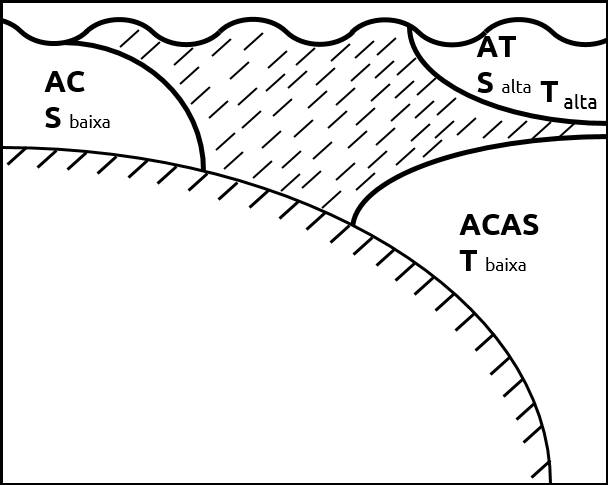
\includegraphics[width=0.5\linewidth]{figuras/massasPCSE.png}
\caption[Massas d'água que preenchem a PCSE]{Esquema gráfico das massas d'água que preenchem a PCSE e suas principais características. A região rachurada representa águas da plataforma continental, que seria a mistura das três massas, mas sem uma definição precisa. Extraído de \cite{castro2015191}.}
    \label{fig:massas_dagua}
\end{figure}

%\section{Divisão da PCSE}
% §.4 explicar as frentes e inserir o termo FTP e  FHS
%\hspace{5mm} Considerando que as diferentes propriedades entre as massas intensificarão os gradientes quase-horizontais de densidade, há então a ocorrência de frentes termohalinas na região \citep{castro2008processos}. Sendo assim, \citep{castro1996correntes} define em seu trabalho a presença de duas frentes na região norte da PCSE: a Frente Térmica Profunda (FTP), associada a intrusão da ACAS, separando a água costeira das águas com origem em regiões mais profundas, e a Frente Halina Superficial (FHS), associada ao encontro entre água tropical e água costeira.
\hspace{5mm} Segundo \cite{castro1996correntes}, há presença de duas frentes na PCSE: a Frente Térmica Profunda (FTP) e a Frente Halina Superficial (FHS). A Frente Térmica Profunda, é caracterizada pela intersecção da termoclina com o fundo, formada na região de encontro entre a ACAS e AC e associada a intrusões pelo fundo das águas transportadas pela CB em direção à costa. Já a Frente Halina Superficial é caracterizada como uma frente de quebra da plataforma, embora não esteja posicionada sobre a quebra da plataforma. Está associada à intrusões das águas da CB e separa, na superfície, a AC da AT.

% §.5 classificacao das regiões e sazonalidade
\hspace{5mm} Embasado em trabalhos anteriores, no conhecimento sobre as propriedades termohalinas da região da Plataforma Continental Norte de São Paulo (PCNSP) e análises de dados hidrográficos, \cite{castro1996correntes} propôs a divisão da plataforma em 3 ambientes (Figura~\ref{fig:pcnsp}), com variação sazonal:

\begin{itemize}
    \item Plataforma Continental Interna: localizada entre a costa e FTP, a PCI varia sazonalmente, possuindo uma largura de 10-30km e um limite externo entre as isóbatas de 20-40m no verão e largura de 40-80km com limite externo entre as isóbatas de 50 e 70m no inverno. Embora possua uma variação sazonal, a PCI tende a ter uma temperatura homogênea tanto na vertical quanto na horizontal;
    \item Plataforma Continental Média: compreendida entre FTP e FHS, é bem definida no verão, com a presença da termoclina sazonal, variando de 10-30km da costa até aproximadamente 60-80km. No inverno, a PCM reduz, compreendo uma região de 40-60km a 60-80km, a partir da costa e
    \item Plataforma Continental Externa: prolongando-se da FHS até a quebra da plataforma continental, entre as isóbatas de 70 e 90m. Possui estratificação vertical bem definida, mas com termoclina mais difusa no verão, e possui pequena variação sazonal de suas propriedades.
\end{itemize}

\begin{figure}[!h]
    \centering
    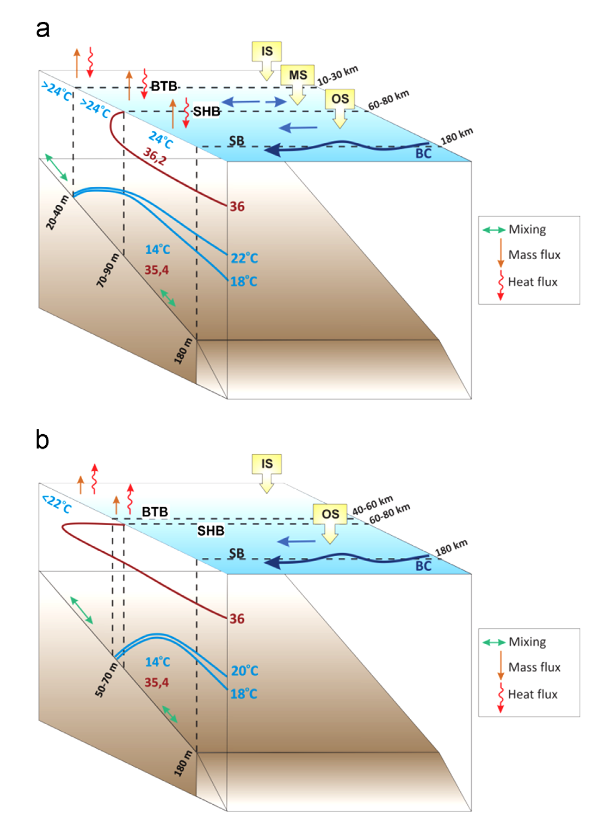
\includegraphics[width=0.65\linewidth]{figuras/divisao_PCNSP.png}
\caption[Divisão da Plataforma Continental de São Paulo]{Esquema da divisão da Plataforma Continental Norte de São Paulo para (a) verão e (b) inverno. IS, MS e OS representam, respectivamente, PCI, PCM e PCE, enquanto que BTB e SHB representam as frentes FTP e FHS. A distância da costa está apresentada em quilômetros e a profundidade em metros. Adaptado de \citep{castro2014summer}.}
    \label{fig:pcnsp}
\end{figure}

% §.6 sazonalidade dos compartimentos
\hspace{5mm} \cite{castro2014summer} idenfitica em seu trabalho que o principal processo da estratiticação da PCI e PCM ao largo de Ubatuba é a variação vertical de densidade, sendo que na PCI é devido a descarga fluvial com águas de baixa salinidade e, na PCM, pela intrusão da ACAS no fundo. Tal variação sazonal pode ser atribuída a outras regiões da PCSE, desde o norte, próximo a Cabo Frio, quanto a sul, próximo a Santa Catarina \citep{cerda2014,brandini2014deep,nogueira2013distribution}.

% §.7 expansão da classificação da plataforma para a PCSE
\hspace{5mm} Desta forma, podemos utilizar a subdivisão da Plataforma Continental em diversas regiões da PCSE \citep{de2003intrusoes,cerda2014}, atentando-se para possíveis particularidades, como no caso de Santa Catarina, onde no verão a subdivisão é adequada, mas no inverno deve-se considerar possíveis intrusões de águas de baixa temperaturas vindas do Rio Grande do Sul \citep{carvalho2010estrutura}.

\section{Circulação na PCSE}
\label{sec:circulation}

% §.8 falar das 4 forçantes: vento, densidade, maré e CB
\hspace{5mm} As correntes na PCSE são forçadas pelos seguintes processos:

\begin{itemize}
    \item Corrente do Brasil (CB): influencia, principalmente, a PCE, ao gerar movimentos devido os meandros e vórtices liberados. Em regiões de plataforma mais estreita, a influência da CB pode ocupar toda a extensão da plataforma \citep{castro2008processos};

    \item Marés: geram correntes perpendiculares à costa, nas regiões mais largas da PCSE, e correntes paralelas à costa em regiões mais estreitas da PCSE \citep{pereira2007numerical}, sendo que a componente M2 é a de energia mais significativa;

    \item Gradientes de Densidade: causado quando águas de origem continental e, portanto, de baixa salinidade, se encontram com as águas da plataforma, de maior salinidade, ocasionando correntes geostróficas paralelas à linha de costa, deixando-a a esquerda do movimento \citep{brink2005coastal} e

    \item Tensão de Cisalhamento do Vento: é a maior forçante de mecanismos de baixa frequência na circulação costeira. O regime de ventos na região Sudeste brasileira é determinado por dois sistemas meterológicos, a Alta Subtropical do Atlântico Sul (ASAS) e Sistemas Frontais \citep{castro1998physical}. A ASAS está relacionada com o regime de vento predominante da PCSE, com ventos de leste e nordeste, que são intensificados no verão. Já os sistemas frontais, ou frentes frias, ocorrem em um período de 6 a 11 dias, formadas ao sul do Brasil e associadas a ventos do quadrante sul \citep{stech1990estudo,stech1992response}.
\end{itemize}

%\begin{figure}[!h]
%    \centering
%    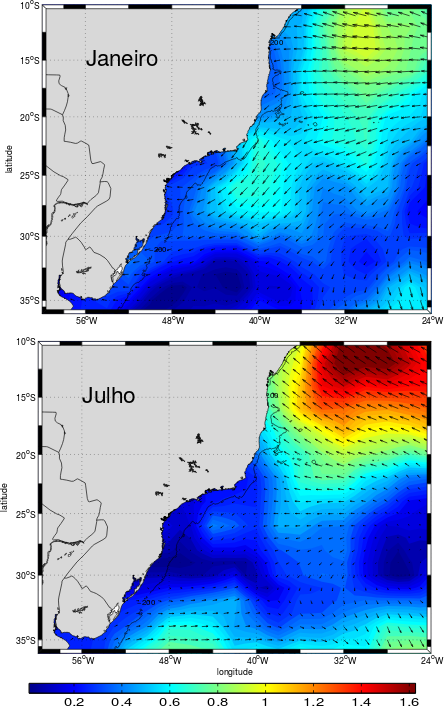
\includegraphics[width=0.8\linewidth]{figuras/campoVento.png}
%\caption[Campo de tensão de cisalhamento do vento.]{Tensão de cisalhamento do vento na região oeste do oceano Atlântico Sul para janeiro e julho, %com a plataforma continental sudesteno centro. Figura extraída de \cite{mazzini2009correntes}.}
%\label{fig:campoVento}
%\end{figure}

% §.9 explicar as forçantes em cada subdivisão
\hspace{5mm} Os movimentos das águas da PCSE são geradas por uma combinação diferente das forçantes citadas, em diferentes regiões da plataforma e em distintas escalas espaciais e temporais \citep{castro1996correntes}. Na plataforma externa, as correntes são forçadas, principalmente, pela Corrente do Brasil \citep{castro2008processos}, com pequenas contribuições da tensão do cisalhamento dos ventos na direção quase paralela às isóbatas locais \citep{dottori2009response}. Já na plataforma média, a forçante predominante é a tensão do cisalhamento dos ventos e a maré, sendo que a influência da Corrente do Brasil só é observada nas regiões mais estretas da plataforma. Por fim, a plataforma interna possui influência das marés, gradientes de densidade e a tensão de cisalhamento do vento.

% §.10 explicar pq focarei somente ne PCI e PCM e somente no vento
\hspace{5mm} Dado que o tema da dissertação do autor será avaliar a influência de ventos anômalos, em eventos raros, sobre a PCSE, a seguir será descrito de forma mais completa a circulação na Plataforma Continental Interna e Média, onde o vento atua com maior influência na circulação.

\section{Circulação na PCI e PCM}

% §.11 principais forcantes na PCI e PCM
\hspace{5mm} Segundo \cite{castro1996correntes}, a circulação em grande parte da plataforma interna é forçada, em diferentes escalas de tempo, pelos ventos, marés e por gradientes de densidade. Sendo que, a maior variância das correntes na PCI e na PCM, foram observadas em duas bandas de frequência, 3-7 e 9-15 dias, associados às oscilações do vento e do nível do mar \citep{castro1998physical}.

% §.12 informacoes sobre PCI (dados in situ e etc)
\hspace{5mm} \cite{castro1996correntes}, ao analisar dados \textit{in situ} na plataforma interna, ao largo de Ubatuba, comprovou a predominância de correntes para SW durante o inverno, com valores típicos da ordem de 0.2 $m.s^{-1}$, havendo eventos de inversão do fluxo para NE, com intensidades da ordem de 0.10 $m.s^{-1}$. Segundo o mesmo autor e demonstrado posteriormente por \cite{dottori2009response}, as componentes paralelas à costa da corrente são essencialmente barotrópica, representando 95$\%$ da variância do primeiro modo ortogonal empírico. Além disso, observou-se que as correntes quase paralelas à costa foram as mais intensas, apresentando uma variabilidade temporal mais energética que as correntes quase perpendiculares.

% jato costeiro, tipico de pci
% \hspace{5mm} jatos costeiros e variabilidade subinercial destes

\hspace{5mm} \cite{valente1999circulaccao} analisou dados correntográficos na plataforma interna, ao largo de Praia Grande e Ubatuba, no litoral Norte de São Paulo. Os pontos a sul da Ilha de São Sebastião apresentaram correntes mais frequentes para N-E, enquanto que os pontos a norte da mesma ilha apresentaram correntes opostas, para S-W. Tal fato foi confirmado por \cite{mazzini2009correntes}, ao analisar correntográficos entre Peruíbe e São Sebastião (SP). Desta forma, pode-se constatar que, durante o verão, há um balanço entre a corrente gerada pela tensão de cisalhamento do vento, para SW, e a corrente gerada pelo gradiente de densidade, para NE, devido a geostrofia.

%-------------------------------------------------------------------------------------------------------

% § transicao entre PCI e PCM, falar sobre castro1996
\hspace{5mm} A principal forçante da circulação da plataforma média são os ventos, havendo coerência significativa entre plataforma interna e média, em oscilações de períodos médios e curtos. A direção predominante dos fluxos na PCM são para SW, com intensidade entre 0.30-0.20 $m.s^{-1}$, havendo inversões para NE mais frequentes do que na PCI. Entretanto, a componente paralela é essencialmente barotrópica e  a componente normal possui um grande cisalhamento vertical, tornando os modos baroclínicos de grande importância \citep{castro1996correntes}.

% §.13 estudos numéricos
\hspace{5mm} Diversos estudos numéricos para avaliar a resposta da plataforma interna aos regimes de ventos foram realizados. \cite{castro1985subtidal} estudou a resposta hidrodinâmica barotrópica da PCSE ao vento climatológico típico de inverno, obtendo como conclusão que as correntes ficam confinadas na plataforma continental com escala de decaimento neperiano de 70-120 km da costa. Ainda neste estudo, foi possível observar que a componente normal à costa é dominada pelo balanço geostrófico e a componente paralela à costa está em balanço friccional, entre a tensão de cisalhamento do vento e a tensão de cisalhamento com o fundo, nas áreas mais costeiras.

\hspace{5mm} As correntes paralelas à costa podem sofrer inversão de sentido, em escala subinercial, devido à passagem de sistemas frontais \citep{stech1992response,dottori2009response}. \cite{coelho2008resposta} estudou a resposta da PCSE a ventos sazonais e sinóticos de verão, obtendo como resultados fluxos para NE na plataforma interna e para SW na plataforma média e externa. O autor utilizou como forçante a passagem de sistemas frontais típicos de verão na região, onde a porção ao sul da Ilha de São Sebastião apresentou a resposta com maiores intensidades a este evento. Com a inversão do regime de ventos na PCSE durante a passagem da frente, observou-se que as correntes na plataforma interna são intensificadas, enquanto que na plataforma média e externa há um enfraquecimento da corrente nas camadas mais superciciais.


% §.17 trabalho do Pedro
\hspace{5mm} \cite{morais2016hidrodinamica}, ao analisar um extenso conjunto de dados e utilizando saídas de modelos numéricos, corrobora com os trabalhos acima apresentados. No entanto, a descarga fluvial ainda não foi devidamente analisada, devido a ausência de dados de vazão dos principais rios e estuários da PCSE, para averiguar seu papel na circulação resultante na PCI e PCM. Ainda assim, espera-se que, em períodos de maior chuva, a descarga fluvial aumente, reduzindo a salinidade das águas da PCI, intensificando o gradiente horizontal de densidade, tendendo a gerar correntes geostróficas que deixam a costa à esquerda do movimento \citep{de2003intrusoes}.


% §.18 componentes de maré de maior importância
\hspace{5mm} \cite{mesquita1983tides} analisaram dados horários de nível do mar para um período de um ano, em Cananéia e Ubatuba, concluindo que as constituintes diurnas dominantes nas estações fora, respectivamente, $O_1$, com 0.110 e 0.109m, e $K_1$, com 0.065 e 0.059. Entre as semi-diurnas, os valores obtidos foram: $M_2$, 0.366 e 0.297m, e $S_2$, com 0.0237 e 0.171m. Todas as constituintes apresentaram rotação anticiclônica, com exceção da $O_1$ e toda a energia proveniente dessas componentes é transportada ao longo da plataforma por ondas de Poincaré e de Kelin \citep{munk1970tides}.

\hspace{5mm} As correntes de maré na PCI são, em geral, uma ordem de grandeza menos intensa do que as correntes geradas pela combinação das forçantes gradiente de densidade e tensão de cisalhamento do vento \citep{castro1996correntes}, sendo que nas proximidades de Santos e no Canal de São Sebastião, \cite{valente1999circulaccao} obteve magnitudes em torno de 0.02 a 0.06 $m.s{-1}$.

\section{Episódios Anômalos}
\label{sec:anomamlousEpisodes}

\hspace{5mm} 

\hspace{5mm} Embora haja períodos em que os ventos predominam de Sul na PCSE, o tempo de
influência deste regime não passa de alguns dias, durante a passagem das frentes frias.
Entretanto, durante o verão de 2014, os ventos associados ao sistema que antes eram de Leste e
Nordeste, passam a ser de Sudoeste, agindo na região costeira por um longo período, como
pode ser observado na Figura~\ref{fig:a701}, onde a direção e intensidade do vento
obtida no \textit{Climate Forecast System Version 2} (CFSv2), durante o período de
01 de Dezembro de 2013 a 28 de Feveiro de 2014. Nota-se que a direção
predominante neste período é do terceiro quadrante (S/SW).

\begin{figure}[!h]
    \centering
    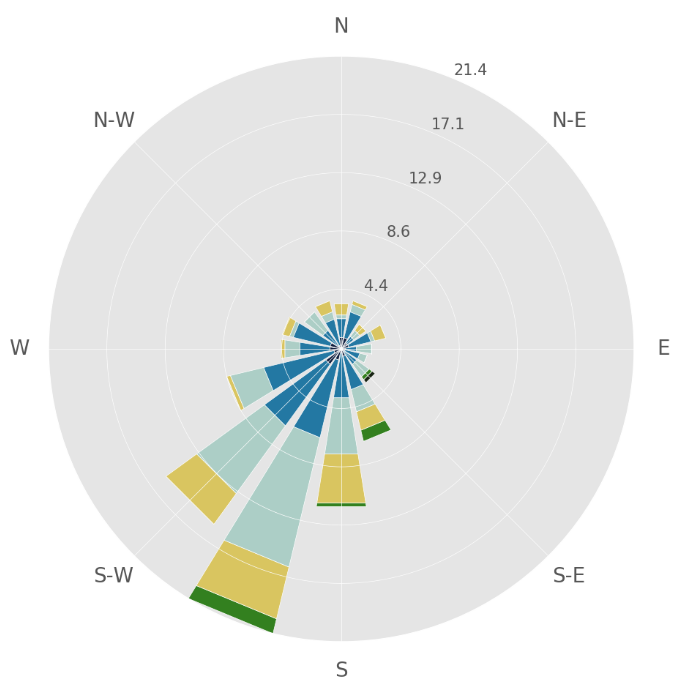
\includegraphics[width=0.65\linewidth]{figuras/windrose_2014CFSv2.png}
\caption[Rosa dos Ventos para Dezembro/2013 a Fevereiro/2014]{Rosa dos ventos para ventos a 10 metros de altura da superfície, extraídos do \textit{Climate Forecast System Version 2} (CFSv2), para o período de Dezembro/2013 a Fevereiro/2014, utilizando-se a conveção meteorológica.}
    \label{fig:a701}
\end{figure}

\hspace{5mm} Com a mudança observada no regime de ventos predominante neste período, a circulação conduzida pelo vento
na plataforma continental interna e média foram alteradas. 
Frente a importância da PCSE, tanto no aspecto de navegação, quanto de
exploração e uso das águas e considerando que as mudanças climáticas poderão
influenciar a frequência de eventos de deslocamento da ASAS, é importante compreender
como a dinâmica da circulação será afetada sob a influência de novos regimes
de vento.

% \hspace{5mm} Com essa mudança no regime de ventos predominante neste
% cenário, a circulação conduzida pelo vento na plataforma muito provavelmente sofreu alterações.
% Frente a importância da PCSE, tanto no aspecto de navegação, quanto de
% exploração e uso das águas e considerando que as mudanças climáticas poderão
% influenciar a frequência de eventos de deslocamento da ASAS, é importante compreender
% como a dinâmica da circulação será afetada sob a influência de novos regimes
% de vento.



\section{Objetivo Geral e Específico}
\label{sec:objectives}

\hspace{5mm} A hipótese científica deste trabalho é que os ventos do quadrante Sul, associados
ao deslocamento da Alta Subtropical do Atlântico Sul para oeste de sua posição
climatológica, alterou de forma efetiva a dinâmica das águas da Plataforma
Continental Sudeste, durante o verão de 2014.

\hspace{5mm} Para tanto, este trabalho tem como objetivo analisar dados de vento de reanálise de banco de dados públicos, a fim de elaborar uma climatologia para os meses de verão (Dezembro, Janeiro e Fevereiro). Esta climatologia será utilizada, então, em um experimento controle para modelar a circulação da Plataforma Continental Interna e Média Sudeste. 
Outros experimentos serão então realizados, utilizando ventos de saída de modelos regionais para o verão de 2014, a fim de comparar a circulação gerada no controle com os cenários de ventos anômalos na região. Mais especificamente, pretende-se:

\begin{itemize}
    \item Determinar a climatologia de ventos para os meses de verão (Dezembro, Janeiro, Fevereiro e Março) na PCSE;
    % \bigskip
    \item Implementar o modelo hidrodinâmico na PCSE para estudar as correntes geradas pelo vento local;
    % \bigskip
    \item Verificar as mudanças geradas pela alteração do regime de ventos.
    % \bigskip
\end{itemize}
 % Introduction

% \lhead{\emph{Anexo B - Materiais e Métodos}} 
% \chapter{Materiais e Métodos}

\section{Climatologia de Ventos}
\label{sec:windClimatology}

\hspace{6mm} Serão utilizados dois tipos de dados (Tabela~\ref{tab:dataset}) da componente
zonal e meridional do vento a 10 metros de altura da superfície: dados de reanálise e
dados \textit{in situ}. Os dados de reanálises serão extraídos do \textit{Climate
Forecast System Reanalysis} (CFSR), para os meses de Dezembro, Janeiro, Fevereiro e
Março, compreendidos entre 1979 e 2010. Quanto aos dados \textit{in situ}
serão extraídos do Programa Nacional de Boias (PNBOIA) das bóias 157597 (Santa Catarina)
e 69009 (Cabo Frio). Mais informações sobre os conjuntos de reanálise são descritos em
\cite{Saha2010} e \cite{Berrisford2011}.

% Inicialmente serão extraídos dados da componente zonal e meridional
% do vento a 10 metros de altura da superfície, a fim de comparar com dados
% \textit{in situ}, para determinação de qual conjunto de dados melhor representa
% o cenário de ventos da PCSE. Em seguida, serão extraídos os mesmos dados de vento
% para os meses de Janeiro, Fevereiro e Março entre 1979 e 2010. Estes dados serão
% então utilizados para elaboração da climatologia de ventos da região. Os conjuntos
% de dados a serem utilizados estão apresentados de forma mais detalhada na
% Tabela~\ref{tab:dataset}.
\bigskip
\begin{center}
\begin{tablehere}
\caption{Conjunto de dados que serão utilizados.}
\label{tab:dataset}
\begin{tabular}{|c|c|c|}

\hline
\textbf{Conjunto de Dados}                   & \textbf{Tipo}    & \textbf{Região}      \\ \hline
CFSR    & Reanálise        & -20$^o$/-30$^o$; -40$^o$/-50$^o$ \\ \hline
PNBOIA - 157597 & \textit{in situ} & -28.51$^o$; -47.39$^o$     \\ \hline
PNBOIA - 69009  & \textit{in situ} & -22.98$^o$; -42.10$^o$     \\ \hline
\end{tabular}
\end{tablehere}
\bigskip
\end{center}

\section{Modelagem Numérica da Circulação}
\label{sec:numericalModelling}

% roteiro:
% apresentar secom
% apresentar falar de algumas coisas: grade, condições de contorno (fechada: no slip boundary, aberta: elevação/maré?)
% falar dos dados que serão implementados: batimetria, vento, TS, maré e outros

\hspace{5mm} Para analisar a circulação na região de interesse, será implementado o modelo \textit{Stevens
Estuarine and Coastal Ocean Model} (sECOM), incluindo as forçantes vento, maré e gradiente de densidade,
sendo este modelo um variante do \textit{Princeton Ocean Model} (POM) \citep{Blumberg1987}.

\hspace{5mm} Este é um modelo numérico de circulação costeira e estuarina, tridimensional, que utiliza equações primitivas empregando
grades C de Arakawa em conjunto com o sistema de coordenadas $\sigma$ na vertical, no processo de discretização.
Dentre os módulos existentes no sECOM, neste trabalho será utilizado somente o Módulo Hidrodinâmico,
descrito no item a seguir.


\subsection{Módulo Hidrodinâmico}
\label{sub:hydrodynamicModule}

\hspace{5mm} As equações deste módulo descrevem os campos de velocidade, elevação da superfície livre,
temperatura e salinidade. Para isso, utiliza duas aproximações:
\begin{enumerate*}[label=(\alph*)]
  \item aproximação hidrostática, que considera o equilíbrio entre o peso do fluido e a força de gradiente de
  pressão na vertical e
  \item aproximação de Boussinesq, ignorando as variações de densidade, exceto quando são multiplicadas pela
  gravidade.
\end{enumerate*}
O conjunto de equações resolvido pelo modelo envolve a conversação de massa, momento, calor e
sal, em função da velocidade, temperatura ($T$) e salinidade ($S$) \citep{Harbor1999}.

\hspace{5mm} Além das equações citadas, o módulo hidrodinâmico parametriza a turbulência baseado no trabalho de 
\citep{mellor1974hierarchy}, onde os coeficientes de difusão turbulenta são obtidos através do esquema de fechamento turbulento de segunda ordem \cite{mellor1982development}.

\subsection{Domínio}
\label{sub:domain}

% Grade, condições de contorno conhecidas (Reid e Bodine [1968], aberta. no slip boundary condition, fechada)
\hspace{5mm} A grade numérica que será utilizada neste trabalho (Figura~\ref{fig:areaestudo}) foi elaborada
em \cite{pereira2007numerical} e adaptada pelo Laboratório de Hidrodinâmica Costeira (LHiCo), para remoção
das células secas. Trata-se de uma grade ortogonal e curvilínea, com 110 pontos na direção $x$, há
uma resolução horizontal variando de 0.5 km a 5 km nesta direção Na direção $y$, 137 pontos,
com uma resolução horizontal variando de 0.5 km, na parte mais central, a 35 km nas regiões com profundidade
superiores a 2100 m. A resolução vertical é de 37 níveis sigma, sendo $\sigma = 0$ na superfície e $\sigma = -1$
no fundo.

\hspace{5mm} Nos experimentos numéricos será considerada a condição de livre escorregamento
nos contorno laterais fechados, ou seja, próximos a costa. Nos contornos abertos será implementada
a condição radiativa, elaborada por \citep{reid1968numerical}, onde o contorno será forçado
pela elevação da superfície livre do mar influenciada pela maré.


\begin{figure}[!h]
    \centering
    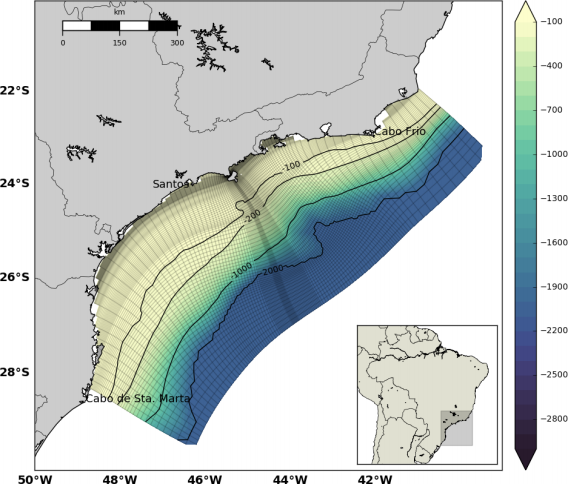
\includegraphics[width=0.7\textwidth]{figuras/grade.png}
\caption[Plataforma Continental Sudeste]{Localização da Plataforma Continental Sudeste, com dados batimétricos fornecidos
pelo Laboratório de Hidrodinâmica Costeira (LHiCo) e grade numérica adaptada de \cite{pereira2007numerical}.}
    \label{fig:areaestudo}
\end{figure}

% condições iniciais está faltando

\subsection{Forçantes}
\label{sub:forcing}


% \hspace{5mm} Batimetria

\hspace{5mm} Os dados de vento serão extraídos do CSFv2, para o meses de Dezembro de 2013 a Março de 2014, que 
serão interpolados espacialmente para a resolução da grade numérica utilizada, preservando-se a resolução
temporal de 6 horas, como disponibilizados os dados.

\hspace{5mm} Serão implementadas a amplitude e fase das componentes semidiurnas de maré,
$M_2$ e $S_2$, que, segundo \citep{mesquita1987harmonic}, são as componentes de maior
relevância na região. Os dados serão extraídos do banco de dados global TPXO 7.2, com
resolução de 1/4 de grau sendo, então, interpolados para os contornos abertos da grade utilizada.
A metodologia completa utilizada pelo TPXO 7.2 pode ser consultada em \citep{Egbert1994}
e \citep{Egbert2002}.

\hspace{5mm} Para os campos de densidade, serão utilizados dados climatológicos de Temperatura
e Salinidade para o verão da PCSE, elaborados por \cite{de2003intrusoes} e disponíveis no
Laboratório de Hidrodinâmica Costeira.


\subsection{Experimentos Numéricos}
\label{sub:numericalExperiments}

\hspace{5mm} Serão realizados dois conjuntos de experimentos numéricos, sendo
\begin{enumerate*}[label=(\alph*)]
  \item um controle, onde será utilizada a climatologia elaborada e
  \item outro com o padrão de ventos anômalos.
\end{enumerate*}
Em todos os experimentos, as forçantes maré e gradiente de densidade serão consideradas.

\hspace{5mm} O tempo de simulação para cada experimento será de três meses (90 dias), compreendendo
o período do fenômeno no ano de 2014, ou seja, de Janeiro a Março. Entretanto, com o objetivo de
aquecer o modelo, serão simulados 7 dias adicionais antes do mês de Dezembro e estes não serão
contemplados nas análises dos dados.

% \lhead{\emph{Capítulo 3 - Resultados Esperados}} 
% \chapter{Resultados Esperados}

\hspace{5mm} Espera-se que, com a climatologia elaborada neste projeto, seja possível reproduzir as feições oceanográficas típicas da plataforma continental interna e média, dominadas pela forçante vento. Com isso, obteremos uma simulação numérica controle para o verão, nos permitindo comparar os experimentos com os campos de ventos anômalos com dados próximos ao real. Desta forma, obteremos uma melhor descrição do efeito do fenômeno na PCSE e as consequências hidrodinâmicas.
% 

%\input{Chapters/Chapter6} % Results and Discussion

%\input{Chapters/Chapter7} % Conclusion

%% ----------------------------------------------------------------
% Now begin the Appendices, including them as separate files

\addtocontents{toc}{\vspace{2em}} % Add a gap in the Contents, for aesthetics

\appendix % Cue to tell LaTeX that the following 'chapters' are Appendices

\chapter{Introdução}

\section{Área de Estudo}
\label{sec:studyArea}

% §.1 localizacao da PCSE e características geográficas, principais cidades, topografia, profundidade de quebra do talue, profundidade media
\hspace{5mm}A Plataforma Continental Sudeste (PCSE), localizada entre Cabo Frio (23ºS), no RJ, e o Cabo de Santa Marta (28º40'S), em SC, é parte integrante do Oceano Atlântico Sudoeste,
estando em constante troca de massa e energia com o oceano profundo adjacente. Sua largura máxima ocorre ao largo de Santos (SP), com cerca de 230km e mais estreita nas extremidades,
chegando a 50km em Cabo Frio (Figura~\ref{fig:areaestudo}). A quebra da plataforma ocorre a cerca de 150km da costa e com profundidade variando entre 120 e 180m \citep{zembruscki1979geomorfologia}. A orientação da linha de costa é NE-SW, sofrendo uma mudança brusca de orientação na região de Cabo Frio (RJ), onde a linha de costa passa a ter uma orientação E-W, sendo que as isóbatas acompanham essa orientação, descrevendo uma topografia suave e com um volume total estimado de 10.000$km^3$, considerando uma profundidade média de 70m \citep{castro1996correntes}.

\hspace{5mm} A PCSE apresenta características típicas de uma plataforma do tipo A ("\textit{wide shelf with shelf-edge western boundary current}"), com a Corrente do Brasil influenciando a parte mais externa da plataforma (sobre a quebra do talude), mas não tendo influência nas regiões mais costeiras \citep{castro2014summer,loder1998western}.

% §.2 importância economica para o Brasil
\hspace{5mm} Devido a sua extensão, a PCSE é uma zona de enorme valor econômico para o Brasil, uma vez que diversos empreedimentos costeiros estão instalados nesta região, como o Porto de Santos, estações de extração de petróleo e gás, indústrias e demais exemplos atrelados ao desenvolvimento do país. Sendo assim, torna-se de suma importância compreendermos os mecanismos que controlam a circulação da plataforma e suas interações, a fim de mitigar quaisquer intervenções, atrópicas ou não, na região.

%\section{Massas de Água da PCSE}

\hspace{5mm} Ao largo da PCSE, a Corrente do Brasil transporta, basicamente, duas massas de água:

\begin{itemize}
    \item Água Tropical (AT), transportada em profundidades de até 200m, possui temperatura superior a 20ºC e salinidade superior a 36 \citep{miranda1982analise} e
\item Água Central do Atlântico Sul (ACAS), transportada abaixo da picnoclina (entre 200 e 600m), com temperatura inferior a 20ºC e salinidade abaixo de 36.40 \citep{miranda1982analise}.
\end{itemize}

\hspace{5mm} Devido a diversos mecanismos, essas massas podem deslocar-se em direção a costa e, devido ao aporte de água doce do continente, a mistura entre as massas resulta na Água Costeira (AC), caracterizada por baixa salinidade. Sendo assim, são três massas d'água que preenchem a PCSE (Figura~\ref{fig:massas_dagua}), onde a AC ocupa a região mais costeira, a AT ocupa níveis mais superficiais da coluna d'água e, por fim, a ACAS ocupa os níveis mais inferiores \citep{emilsson1961shelf,de1979aplicaccao,miranda1982analise,castro1998physical}.

\begin{figure}[!h]
    \centering
    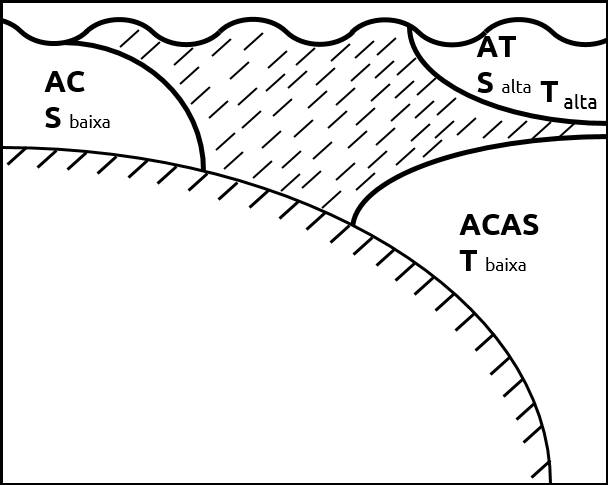
\includegraphics[width=0.5\linewidth]{figuras/massasPCSE.png}
\caption[Massas d'água que preenchem a PCSE]{Esquema gráfico das massas d'água que preenchem a PCSE e suas principais características. A região rachurada representa águas da plataforma continental, que seria a mistura das três massas, mas sem uma definição precisa. Extraído de \cite{castro2015191}.}
    \label{fig:massas_dagua}
\end{figure}

%\section{Divisão da PCSE}
% §.4 explicar as frentes e inserir o termo FTP e  FHS
%\hspace{5mm} Considerando que as diferentes propriedades entre as massas intensificarão os gradientes quase-horizontais de densidade, há então a ocorrência de frentes termohalinas na região \citep{castro2008processos}. Sendo assim, \citep{castro1996correntes} define em seu trabalho a presença de duas frentes na região norte da PCSE: a Frente Térmica Profunda (FTP), associada a intrusão da ACAS, separando a água costeira das águas com origem em regiões mais profundas, e a Frente Halina Superficial (FHS), associada ao encontro entre água tropical e água costeira.
\hspace{5mm} Segundo \cite{castro1996correntes}, há presença de duas frentes na PCSE: a Frente Térmica Profunda (FTP) e a Frente Halina Superficial (FHS). A Frente Térmica Profunda, é caracterizada pela intersecção da termoclina com o fundo, formada na região de encontro entre a ACAS e AC e associada a intrusões pelo fundo das águas transportadas pela CB em direção à costa. Já a Frente Halina Superficial é caracterizada como uma frente de quebra da plataforma, embora não esteja posicionada sobre a quebra da plataforma. Está associada à intrusões das águas da CB e separa, na superfície, a AC da AT.

% §.5 classificacao das regiões e sazonalidade
\hspace{5mm} Embasado em trabalhos anteriores, no conhecimento sobre as propriedades termohalinas da região da Plataforma Continental Norte de São Paulo (PCNSP) e análises de dados hidrográficos, \cite{castro1996correntes} propôs a divisão da plataforma em 3 ambientes (Figura~\ref{fig:pcnsp}), com variação sazonal:

\begin{itemize}
    \item Plataforma Continental Interna: localizada entre a costa e FTP, a PCI varia sazonalmente, possuindo uma largura de 10-30km e um limite externo entre as isóbatas de 20-40m no verão e largura de 40-80km com limite externo entre as isóbatas de 50 e 70m no inverno. Embora possua uma variação sazonal, a PCI tende a ter uma temperatura homogênea tanto na vertical quanto na horizontal;
    \item Plataforma Continental Média: compreendida entre FTP e FHS, é bem definida no verão, com a presença da termoclina sazonal, variando de 10-30km da costa até aproximadamente 60-80km. No inverno, a PCM reduz, compreendo uma região de 40-60km a 60-80km, a partir da costa e
    \item Plataforma Continental Externa: prolongando-se da FHS até a quebra da plataforma continental, entre as isóbatas de 70 e 90m. Possui estratificação vertical bem definida, mas com termoclina mais difusa no verão, e possui pequena variação sazonal de suas propriedades.
\end{itemize}

\begin{figure}[!h]
    \centering
    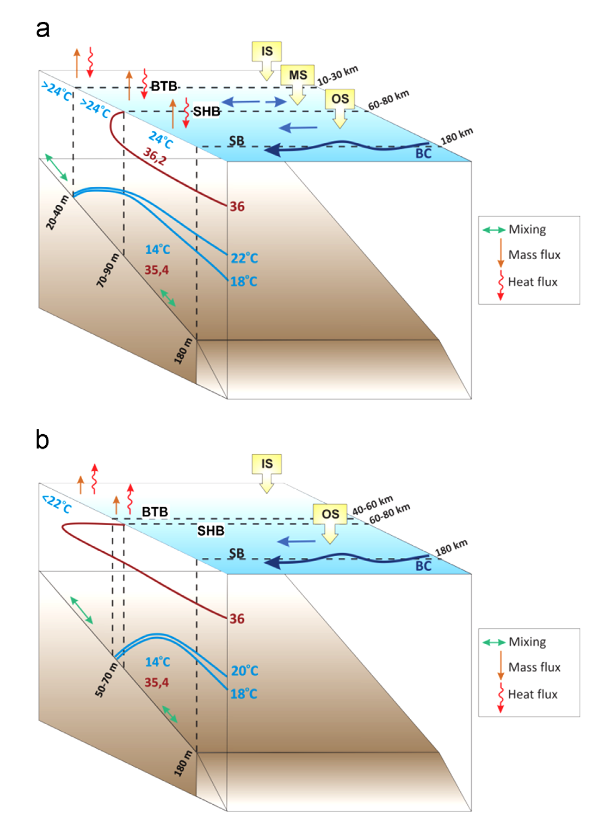
\includegraphics[width=0.65\linewidth]{figuras/divisao_PCNSP.png}
\caption[Divisão da Plataforma Continental de São Paulo]{Esquema da divisão da Plataforma Continental Norte de São Paulo para (a) verão e (b) inverno. IS, MS e OS representam, respectivamente, PCI, PCM e PCE, enquanto que BTB e SHB representam as frentes FTP e FHS. A distância da costa está apresentada em quilômetros e a profundidade em metros. Adaptado de \citep{castro2014summer}.}
    \label{fig:pcnsp}
\end{figure}

% §.6 sazonalidade dos compartimentos
\hspace{5mm} \cite{castro2014summer} idenfitica em seu trabalho que o principal processo da estratiticação da PCI e PCM ao largo de Ubatuba é a variação vertical de densidade, sendo que na PCI é devido a descarga fluvial com águas de baixa salinidade e, na PCM, pela intrusão da ACAS no fundo. Tal variação sazonal pode ser atribuída a outras regiões da PCSE, desde o norte, próximo a Cabo Frio, quanto a sul, próximo a Santa Catarina \citep{cerda2014,brandini2014deep,nogueira2013distribution}.

% §.7 expansão da classificação da plataforma para a PCSE
\hspace{5mm} Desta forma, podemos utilizar a subdivisão da Plataforma Continental em diversas regiões da PCSE \citep{de2003intrusoes,cerda2014}, atentando-se para possíveis particularidades, como no caso de Santa Catarina, onde no verão a subdivisão é adequada, mas no inverno deve-se considerar possíveis intrusões de águas de baixa temperaturas vindas do Rio Grande do Sul \citep{carvalho2010estrutura}.

\section{Circulação na PCSE}
\label{sec:circulation}

% §.8 falar das 4 forçantes: vento, densidade, maré e CB
\hspace{5mm} As correntes na PCSE são forçadas pelos seguintes processos:

\begin{itemize}
    \item Corrente do Brasil (CB): influencia, principalmente, a PCE, ao gerar movimentos devido os meandros e vórtices liberados. Em regiões de plataforma mais estreita, a influência da CB pode ocupar toda a extensão da plataforma \citep{castro2008processos};

    \item Marés: geram correntes perpendiculares à costa, nas regiões mais largas da PCSE, e correntes paralelas à costa em regiões mais estreitas da PCSE \citep{pereira2007numerical}, sendo que a componente M2 é a de energia mais significativa;

    \item Gradientes de Densidade: causado quando águas de origem continental e, portanto, de baixa salinidade, se encontram com as águas da plataforma, de maior salinidade, ocasionando correntes geostróficas paralelas à linha de costa, deixando-a a esquerda do movimento \citep{brink2005coastal} e

    \item Tensão de Cisalhamento do Vento: é a maior forçante de mecanismos de baixa frequência na circulação costeira. O regime de ventos na região Sudeste brasileira é determinado por dois sistemas meterológicos, a Alta Subtropical do Atlântico Sul (ASAS) e Sistemas Frontais \citep{castro1998physical}. A ASAS está relacionada com o regime de vento predominante da PCSE, com ventos de leste e nordeste, que são intensificados no verão. Já os sistemas frontais, ou frentes frias, ocorrem em um período de 6 a 11 dias, formadas ao sul do Brasil e associadas a ventos do quadrante sul \citep{stech1990estudo,stech1992response}.
\end{itemize}

%\begin{figure}[!h]
%    \centering
%    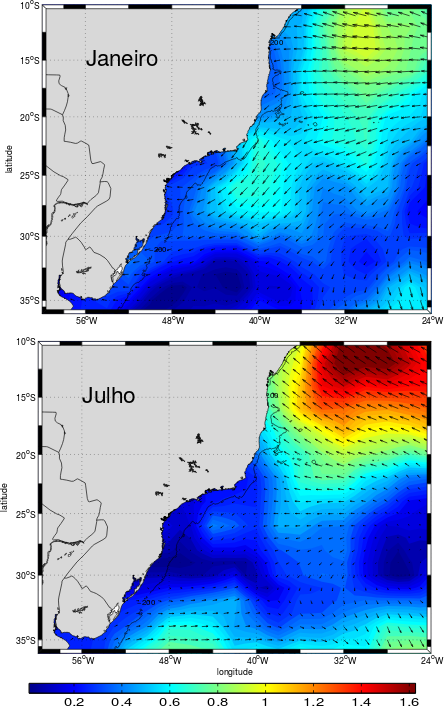
\includegraphics[width=0.8\linewidth]{figuras/campoVento.png}
%\caption[Campo de tensão de cisalhamento do vento.]{Tensão de cisalhamento do vento na região oeste do oceano Atlântico Sul para janeiro e julho, %com a plataforma continental sudesteno centro. Figura extraída de \cite{mazzini2009correntes}.}
%\label{fig:campoVento}
%\end{figure}

% §.9 explicar as forçantes em cada subdivisão
\hspace{5mm} Os movimentos das águas da PCSE são geradas por uma combinação diferente das forçantes citadas, em diferentes regiões da plataforma e em distintas escalas espaciais e temporais \citep{castro1996correntes}. Na plataforma externa, as correntes são forçadas, principalmente, pela Corrente do Brasil \citep{castro2008processos}, com pequenas contribuições da tensão do cisalhamento dos ventos na direção quase paralela às isóbatas locais \citep{dottori2009response}. Já na plataforma média, a forçante predominante é a tensão do cisalhamento dos ventos e a maré, sendo que a influência da Corrente do Brasil só é observada nas regiões mais estretas da plataforma. Por fim, a plataforma interna possui influência das marés, gradientes de densidade e a tensão de cisalhamento do vento.

% §.10 explicar pq focarei somente ne PCI e PCM e somente no vento
\hspace{5mm} Dado que o tema da dissertação do autor será avaliar a influência de ventos anômalos, em eventos raros, sobre a PCSE, a seguir será descrito de forma mais completa a circulação na Plataforma Continental Interna e Média, onde o vento atua com maior influência na circulação.

\section{Circulação na PCI e PCM}

% §.11 principais forcantes na PCI e PCM
\hspace{5mm} Segundo \cite{castro1996correntes}, a circulação em grande parte da plataforma interna é forçada, em diferentes escalas de tempo, pelos ventos, marés e por gradientes de densidade. Sendo que, a maior variância das correntes na PCI e na PCM, foram observadas em duas bandas de frequência, 3-7 e 9-15 dias, associados às oscilações do vento e do nível do mar \citep{castro1998physical}.

% §.12 informacoes sobre PCI (dados in situ e etc)
\hspace{5mm} \cite{castro1996correntes}, ao analisar dados \textit{in situ} na plataforma interna, ao largo de Ubatuba, comprovou a predominância de correntes para SW durante o inverno, com valores típicos da ordem de 0.2 $m.s^{-1}$, havendo eventos de inversão do fluxo para NE, com intensidades da ordem de 0.10 $m.s^{-1}$. Segundo o mesmo autor e demonstrado posteriormente por \cite{dottori2009response}, as componentes paralelas à costa da corrente são essencialmente barotrópica, representando 95$\%$ da variância do primeiro modo ortogonal empírico. Além disso, observou-se que as correntes quase paralelas à costa foram as mais intensas, apresentando uma variabilidade temporal mais energética que as correntes quase perpendiculares.

% jato costeiro, tipico de pci
% \hspace{5mm} jatos costeiros e variabilidade subinercial destes

\hspace{5mm} \cite{valente1999circulaccao} analisou dados correntográficos na plataforma interna, ao largo de Praia Grande e Ubatuba, no litoral Norte de São Paulo. Os pontos a sul da Ilha de São Sebastião apresentaram correntes mais frequentes para N-E, enquanto que os pontos a norte da mesma ilha apresentaram correntes opostas, para S-W. Tal fato foi confirmado por \cite{mazzini2009correntes}, ao analisar correntográficos entre Peruíbe e São Sebastião (SP). Desta forma, pode-se constatar que, durante o verão, há um balanço entre a corrente gerada pela tensão de cisalhamento do vento, para SW, e a corrente gerada pelo gradiente de densidade, para NE, devido a geostrofia.

%-------------------------------------------------------------------------------------------------------

% § transicao entre PCI e PCM, falar sobre castro1996
\hspace{5mm} A principal forçante da circulação da plataforma média são os ventos, havendo coerência significativa entre plataforma interna e média, em oscilações de períodos médios e curtos. A direção predominante dos fluxos na PCM são para SW, com intensidade entre 0.30-0.20 $m.s^{-1}$, havendo inversões para NE mais frequentes do que na PCI. Entretanto, a componente paralela é essencialmente barotrópica e  a componente normal possui um grande cisalhamento vertical, tornando os modos baroclínicos de grande importância \citep{castro1996correntes}.

% §.13 estudos numéricos
\hspace{5mm} Diversos estudos numéricos para avaliar a resposta da plataforma interna aos regimes de ventos foram realizados. \cite{castro1985subtidal} estudou a resposta hidrodinâmica barotrópica da PCSE ao vento climatológico típico de inverno, obtendo como conclusão que as correntes ficam confinadas na plataforma continental com escala de decaimento neperiano de 70-120 km da costa. Ainda neste estudo, foi possível observar que a componente normal à costa é dominada pelo balanço geostrófico e a componente paralela à costa está em balanço friccional, entre a tensão de cisalhamento do vento e a tensão de cisalhamento com o fundo, nas áreas mais costeiras.

\hspace{5mm} As correntes paralelas à costa podem sofrer inversão de sentido, em escala subinercial, devido à passagem de sistemas frontais \citep{stech1992response,dottori2009response}. \cite{coelho2008resposta} estudou a resposta da PCSE a ventos sazonais e sinóticos de verão, obtendo como resultados fluxos para NE na plataforma interna e para SW na plataforma média e externa. O autor utilizou como forçante a passagem de sistemas frontais típicos de verão na região, onde a porção ao sul da Ilha de São Sebastião apresentou a resposta com maiores intensidades a este evento. Com a inversão do regime de ventos na PCSE durante a passagem da frente, observou-se que as correntes na plataforma interna são intensificadas, enquanto que na plataforma média e externa há um enfraquecimento da corrente nas camadas mais superciciais.


% §.17 trabalho do Pedro
\hspace{5mm} \cite{morais2016hidrodinamica}, ao analisar um extenso conjunto de dados e utilizando saídas de modelos numéricos, corrobora com os trabalhos acima apresentados. No entanto, a descarga fluvial ainda não foi devidamente analisada, devido a ausência de dados de vazão dos principais rios e estuários da PCSE, para averiguar seu papel na circulação resultante na PCI e PCM. Ainda assim, espera-se que, em períodos de maior chuva, a descarga fluvial aumente, reduzindo a salinidade das águas da PCI, intensificando o gradiente horizontal de densidade, tendendo a gerar correntes geostróficas que deixam a costa à esquerda do movimento \citep{de2003intrusoes}.


% §.18 componentes de maré de maior importância
\hspace{5mm} \cite{mesquita1983tides} analisaram dados horários de nível do mar para um período de um ano, em Cananéia e Ubatuba, concluindo que as constituintes diurnas dominantes nas estações fora, respectivamente, $O_1$, com 0.110 e 0.109m, e $K_1$, com 0.065 e 0.059. Entre as semi-diurnas, os valores obtidos foram: $M_2$, 0.366 e 0.297m, e $S_2$, com 0.0237 e 0.171m. Todas as constituintes apresentaram rotação anticiclônica, com exceção da $O_1$ e toda a energia proveniente dessas componentes é transportada ao longo da plataforma por ondas de Poincaré e de Kelin \citep{munk1970tides}.

\hspace{5mm} As correntes de maré na PCI são, em geral, uma ordem de grandeza menos intensa do que as correntes geradas pela combinação das forçantes gradiente de densidade e tensão de cisalhamento do vento \citep{castro1996correntes}, sendo que nas proximidades de Santos e no Canal de São Sebastião, \cite{valente1999circulaccao} obteve magnitudes em torno de 0.02 a 0.06 $m.s{-1}$.

\section{Episódios Anômalos}
\label{sec:anomamlousEpisodes}

\hspace{5mm} 

\hspace{5mm} Embora haja períodos em que os ventos predominam de Sul na PCSE, o tempo de
influência deste regime não passa de alguns dias, durante a passagem das frentes frias.
Entretanto, durante o verão de 2014, os ventos associados ao sistema que antes eram de Leste e
Nordeste, passam a ser de Sudoeste, agindo na região costeira por um longo período, como
pode ser observado na Figura~\ref{fig:a701}, onde a direção e intensidade do vento
obtida no \textit{Climate Forecast System Version 2} (CFSv2), durante o período de
01 de Dezembro de 2013 a 28 de Feveiro de 2014. Nota-se que a direção
predominante neste período é do terceiro quadrante (S/SW).

\begin{figure}[!h]
    \centering
    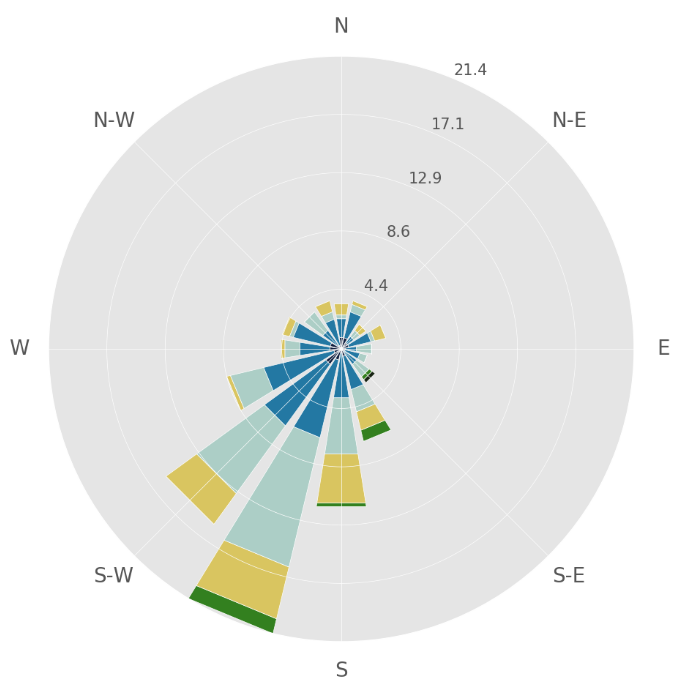
\includegraphics[width=0.65\linewidth]{figuras/windrose_2014CFSv2.png}
\caption[Rosa dos Ventos para Dezembro/2013 a Fevereiro/2014]{Rosa dos ventos para ventos a 10 metros de altura da superfície, extraídos do \textit{Climate Forecast System Version 2} (CFSv2), para o período de Dezembro/2013 a Fevereiro/2014, utilizando-se a conveção meteorológica.}
    \label{fig:a701}
\end{figure}

\hspace{5mm} Com a mudança observada no regime de ventos predominante neste período, a circulação conduzida pelo vento
na plataforma continental interna e média foram alteradas. 
Frente a importância da PCSE, tanto no aspecto de navegação, quanto de
exploração e uso das águas e considerando que as mudanças climáticas poderão
influenciar a frequência de eventos de deslocamento da ASAS, é importante compreender
como a dinâmica da circulação será afetada sob a influência de novos regimes
de vento.

% \hspace{5mm} Com essa mudança no regime de ventos predominante neste
% cenário, a circulação conduzida pelo vento na plataforma muito provavelmente sofreu alterações.
% Frente a importância da PCSE, tanto no aspecto de navegação, quanto de
% exploração e uso das águas e considerando que as mudanças climáticas poderão
% influenciar a frequência de eventos de deslocamento da ASAS, é importante compreender
% como a dinâmica da circulação será afetada sob a influência de novos regimes
% de vento.



\section{Objetivo Geral e Específico}
\label{sec:objectives}

\hspace{5mm} A hipótese científica deste trabalho é que os ventos do quadrante Sul, associados
ao deslocamento da Alta Subtropical do Atlântico Sul para oeste de sua posição
climatológica, alterou de forma efetiva a dinâmica das águas da Plataforma
Continental Sudeste, durante o verão de 2014.

\hspace{5mm} Para tanto, este trabalho tem como objetivo analisar dados de vento de reanálise de banco de dados públicos, a fim de elaborar uma climatologia para os meses de verão (Dezembro, Janeiro e Fevereiro). Esta climatologia será utilizada, então, em um experimento controle para modelar a circulação da Plataforma Continental Interna e Média Sudeste. 
Outros experimentos serão então realizados, utilizando ventos de saída de modelos regionais para o verão de 2014, a fim de comparar a circulação gerada no controle com os cenários de ventos anômalos na região. Mais especificamente, pretende-se:

\begin{itemize}
    \item Determinar a climatologia de ventos para os meses de verão (Dezembro, Janeiro, Fevereiro e Março) na PCSE;
    % \bigskip
    \item Implementar o modelo hidrodinâmico na PCSE para estudar as correntes geradas pelo vento local;
    % \bigskip
    \item Verificar as mudanças geradas pela alteração do regime de ventos.
    % \bigskip
\end{itemize}
	% Appendix Title

\chapter{Materiais e Métodos}

\section{Climatologia de Ventos}
\label{sec:windClimatology}

\hspace{6mm} Serão utilizados dois tipos de dados (Tabela~\ref{tab:dataset}) da componente
zonal e meridional do vento a 10 metros de altura da superfície: dados de reanálise e
dados \textit{in situ}. Os dados de reanálises serão extraídos do \textit{Climate
Forecast System Reanalysis} (CFSR), para os meses de Dezembro, Janeiro, Fevereiro e
Março, compreendidos entre 1979 e 2010. Quanto aos dados \textit{in situ}
serão extraídos do Programa Nacional de Boias (PNBOIA) das bóias 157597 (Santa Catarina)
e 69009 (Cabo Frio). Mais informações sobre os conjuntos de reanálise são descritos em
\cite{Saha2010} e \cite{Berrisford2011}.

% Inicialmente serão extraídos dados da componente zonal e meridional
% do vento a 10 metros de altura da superfície, a fim de comparar com dados
% \textit{in situ}, para determinação de qual conjunto de dados melhor representa
% o cenário de ventos da PCSE. Em seguida, serão extraídos os mesmos dados de vento
% para os meses de Janeiro, Fevereiro e Março entre 1979 e 2010. Estes dados serão
% então utilizados para elaboração da climatologia de ventos da região. Os conjuntos
% de dados a serem utilizados estão apresentados de forma mais detalhada na
% Tabela~\ref{tab:dataset}.
\bigskip
\begin{center}
\begin{tablehere}
\caption{Conjunto de dados que serão utilizados.}
\label{tab:dataset}
\begin{tabular}{|c|c|c|}

\hline
\textbf{Conjunto de Dados}                   & \textbf{Tipo}    & \textbf{Região}      \\ \hline
CFSR    & Reanálise        & -20$^o$/-30$^o$; -40$^o$/-50$^o$ \\ \hline
PNBOIA - 157597 & \textit{in situ} & -28.51$^o$; -47.39$^o$     \\ \hline
PNBOIA - 69009  & \textit{in situ} & -22.98$^o$; -42.10$^o$     \\ \hline
\end{tabular}
\end{tablehere}
\bigskip
\end{center}

\section{Modelagem Numérica da Circulação}
\label{sec:numericalModelling}

% roteiro:
% apresentar secom
% apresentar falar de algumas coisas: grade, condições de contorno (fechada: no slip boundary, aberta: elevação/maré?)
% falar dos dados que serão implementados: batimetria, vento, TS, maré e outros

\hspace{5mm} Para analisar a circulação na região de interesse, será implementado o modelo \textit{Stevens
Estuarine and Coastal Ocean Model} (sECOM), incluindo as forçantes vento, maré e gradiente de densidade,
sendo este modelo um variante do \textit{Princeton Ocean Model} (POM) \citep{Blumberg1987}.

\hspace{5mm} Este é um modelo numérico de circulação costeira e estuarina, tridimensional, que utiliza equações primitivas empregando
grades C de Arakawa em conjunto com o sistema de coordenadas $\sigma$ na vertical, no processo de discretização.
Dentre os módulos existentes no sECOM, neste trabalho será utilizado somente o Módulo Hidrodinâmico,
descrito no item a seguir.


\subsection{Módulo Hidrodinâmico}
\label{sub:hydrodynamicModule}

\hspace{5mm} As equações deste módulo descrevem os campos de velocidade, elevação da superfície livre,
temperatura e salinidade. Para isso, utiliza duas aproximações:
\begin{enumerate*}[label=(\alph*)]
  \item aproximação hidrostática, que considera o equilíbrio entre o peso do fluido e a força de gradiente de
  pressão na vertical e
  \item aproximação de Boussinesq, ignorando as variações de densidade, exceto quando são multiplicadas pela
  gravidade.
\end{enumerate*}
O conjunto de equações resolvido pelo modelo envolve a conversação de massa, momento, calor e
sal, em função da velocidade, temperatura ($T$) e salinidade ($S$) \citep{Harbor1999}.

\hspace{5mm} Além das equações citadas, o módulo hidrodinâmico parametriza a turbulência baseado no trabalho de 
\citep{mellor1974hierarchy}, onde os coeficientes de difusão turbulenta são obtidos através do esquema de fechamento turbulento de segunda ordem \cite{mellor1982development}.

\subsection{Domínio}
\label{sub:domain}

% Grade, condições de contorno conhecidas (Reid e Bodine [1968], aberta. no slip boundary condition, fechada)
\hspace{5mm} A grade numérica que será utilizada neste trabalho (Figura~\ref{fig:areaestudo}) foi elaborada
em \cite{pereira2007numerical} e adaptada pelo Laboratório de Hidrodinâmica Costeira (LHiCo), para remoção
das células secas. Trata-se de uma grade ortogonal e curvilínea, com 110 pontos na direção $x$, há
uma resolução horizontal variando de 0.5 km a 5 km nesta direção Na direção $y$, 137 pontos,
com uma resolução horizontal variando de 0.5 km, na parte mais central, a 35 km nas regiões com profundidade
superiores a 2100 m. A resolução vertical é de 37 níveis sigma, sendo $\sigma = 0$ na superfície e $\sigma = -1$
no fundo.

\hspace{5mm} Nos experimentos numéricos será considerada a condição de livre escorregamento
nos contorno laterais fechados, ou seja, próximos a costa. Nos contornos abertos será implementada
a condição radiativa, elaborada por \citep{reid1968numerical}, onde o contorno será forçado
pela elevação da superfície livre do mar influenciada pela maré.


\begin{figure}[!h]
    \centering
    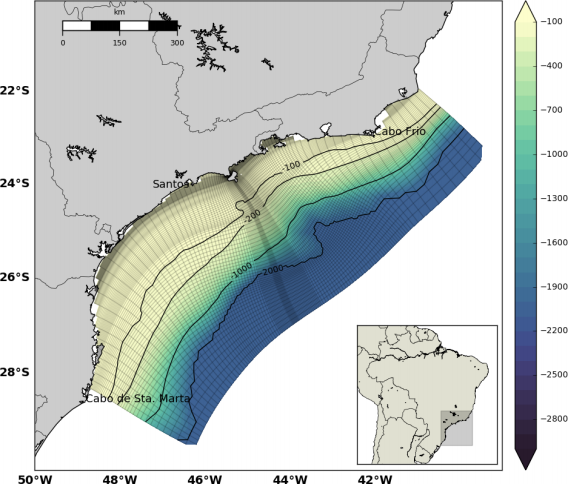
\includegraphics[width=0.7\textwidth]{figuras/grade.png}
\caption[Plataforma Continental Sudeste]{Localização da Plataforma Continental Sudeste, com dados batimétricos fornecidos
pelo Laboratório de Hidrodinâmica Costeira (LHiCo) e grade numérica adaptada de \cite{pereira2007numerical}.}
    \label{fig:areaestudo}
\end{figure}

% condições iniciais está faltando

\subsection{Forçantes}
\label{sub:forcing}


% \hspace{5mm} Batimetria

\hspace{5mm} Os dados de vento serão extraídos do CSFv2, para o meses de Dezembro de 2013 a Março de 2014, que 
serão interpolados espacialmente para a resolução da grade numérica utilizada, preservando-se a resolução
temporal de 6 horas, como disponibilizados os dados.

\hspace{5mm} Serão implementadas a amplitude e fase das componentes semidiurnas de maré,
$M_2$ e $S_2$, que, segundo \citep{mesquita1987harmonic}, são as componentes de maior
relevância na região. Os dados serão extraídos do banco de dados global TPXO 7.2, com
resolução de 1/4 de grau sendo, então, interpolados para os contornos abertos da grade utilizada.
A metodologia completa utilizada pelo TPXO 7.2 pode ser consultada em \citep{Egbert1994}
e \citep{Egbert2002}.

\hspace{5mm} Para os campos de densidade, serão utilizados dados climatológicos de Temperatura
e Salinidade para o verão da PCSE, elaborados por \cite{de2003intrusoes} e disponíveis no
Laboratório de Hidrodinâmica Costeira.


\subsection{Experimentos Numéricos}
\label{sub:numericalExperiments}

\hspace{5mm} Serão realizados dois conjuntos de experimentos numéricos, sendo
\begin{enumerate*}[label=(\alph*)]
  \item um controle, onde será utilizada a climatologia elaborada e
  \item outro com o padrão de ventos anômalos.
\end{enumerate*}
Em todos os experimentos, as forçantes maré e gradiente de densidade serão consideradas.

\hspace{5mm} O tempo de simulação para cada experimento será de três meses (90 dias), compreendendo
o período do fenômeno no ano de 2014, ou seja, de Janeiro a Março. Entretanto, com o objetivo de
aquecer o modelo, serão simulados 7 dias adicionais antes do mês de Dezembro e estes não serão
contemplados nas análises dos dados. % Appendix Title

%\input{Appendices/AppendixC} % Appendix Title

\addtocontents{toc}{\vspace{2em}}  % Add a gap in the Contents, for aesthetics
\backmatter

%% ----------------------------------------------------------------
\label{Bibliography}
\lhead{\emph{Bibliografia}}  % Change the left side page header to "Bibliography"
\bibliographystyle{chicago}  % Use the "unsrtnat" BibTeX style for formatting the Bibliography
\bibliography{Bibliography}  % The references (bibliography) information are stored in the file named "Bibliography.bib"

\end{document}  % The End
%% ----------------------------------------------------------------